\documentclass{beamer}
\usepackage[utf8]{inputenc}

\usetheme{Madrid}
\usecolortheme{default}
\useinnertheme{circles}

\definecolor{Logo1}{rgb}{0.208, 0.2865, 0.373}
\definecolor{Logo2}{rgb}{0.000, 0.674, 0.863}

\setbeamercolor*{palette primary}{bg=Logo1, fg=white}
\setbeamercolor*{palette secondary}{bg=Logo2, fg=white}
\setbeamercolor*{palette tertiary}{bg=white, fg=Logo1}
\setbeamercolor*{palette quaternary}{bg=Logo1,fg=white}
\setbeamercolor{structure}{fg=Logo1} % itemize, enumerate, etc
\setbeamercolor{section in toc}{fg=Logo1} % TOC sections

\usepackage{graphicx,animate}
%------------------------------------------------------------
%This block of code defines the information to appear in the
%Title page
\title[Linear Algebra] %optional
{Matrices and Gaussian Elimination}

\subtitle{Lecture 1}

\author[11910803@mail.sustech.edu.cn] % (optional)
{
    Zhang Ce
}

\institute[] % (optional)
{
    Department of Electrical and Electronic Engineering\\
    Southern University of Science and Technology
}

\date[2021.9.26] % (optional)
{2021.9.26}


%End of title page configuration block
%------------------------------------------------------------



%------------------------------------------------------------
%The next block of commands puts the table of contents at the
%beginning of each section and highlights the current section:

\AtBeginSection[]
{
\begin{frame}
    \frametitle{Table of Contents}
    \tableofcontents[currentsection]
\end{frame}
}
%------------------------------------------------------------


\begin{document}

%The next statement creates the title page.
\frame{\titlepage}


%---------------------------------------------------------
%This block of code is for the table of contents after
%the title page
\begin{frame}
\frametitle{Table of Contents}
\tableofcontents
\end{frame}
%---------------------------------------------------------

\section{Introduction to the Whole Course}

\begin{frame}{About Peer Supporting Class...}
\textbf{Peer Supporting Class} is a program created by the Student Study Centre of SUSTech. This program invites some students to teach several major courses for freshmen.

Courses involved: Linear Algebra (here), Calculus, General Physics, Java.

\begin{figure}
    \centering
    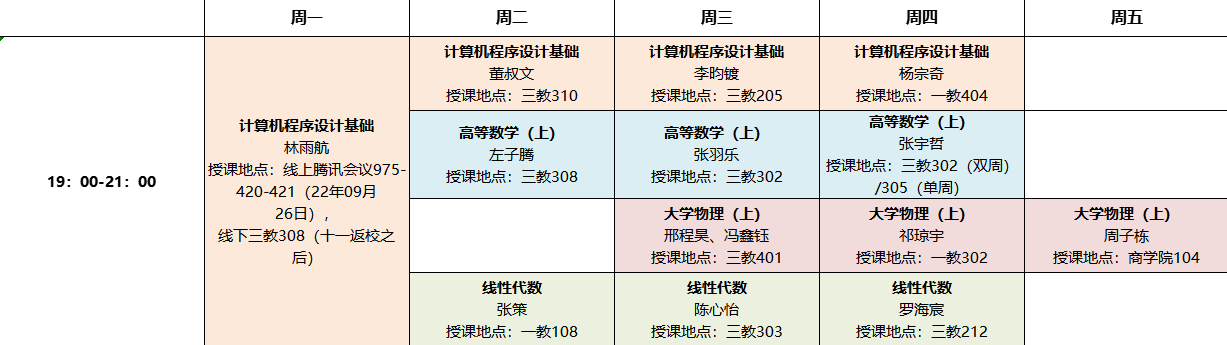
\includegraphics[width=0.75\textwidth]{arrangement.png}
\end{figure}

Come here if you want to learn more and get better grades in these courses, but to be careful with your time arrangement. Feel free to attend these classes, no scores will be graded here!

\end{frame}

\begin{frame}{QQ Group}
\begin{figure}
    \centering
    
\includegraphics[width=0.3\textwidth]{QR.jpg}
\end{figure}
\textbf{Please scan the QR code above to enter the QQ group.}

Feel free to ask questions in that QQ group. Help others and improve yourself by participating the discussions. Some review slides will be released in QQ group before the exam, hope these materials can help you!

\end{frame}

\begin{frame}{About Me...}
\begin{itemize}
    \item \textbf{Name}: Zhang Ce
    \item \textbf{Grade}: 3
    \item \textbf{Department}: Electrical and Electronic Engineering
    \item \textbf{Major}: Communication Engineering
    \item \textbf{E-Mail}: 11910803@mail.sustech.edu.cn
    \item Get $100 (A+)$ in Linear Algebra A, Fall 2019. \\
    \vspace{3pt}
    Midterm Exam: $100/100$ \qquad Final Exam: $100+/110$
    \item Contact me directly on QQ (recommended) or email if you have problems on this course or issues about major selection.
    \item I'm not your instructor, I'm just one of your schoolmates. I will try my best to prepare and give my lectures, and I can always learn from you at the same time.
\end{itemize}

\end{frame}

\begin{frame}{About This Course...}
\begin{itemize}
    \item \textbf{Course Name}: Linear Algebra A / B
    \item \textbf{Course Code}: MA107A / MA107B
    \item \textbf{Course Category}: GR (General Education Required Course)
    \item \textbf{Class Hours}: 64 \qquad \textbf{Total Credits}: 4
    \item \textbf{Assessment}: '334' Grading System \quad $60\%$ to pass this course\\
        \vspace{5pt}
        $30\%$ Regular Performance\\
        \vspace{3pt}
        \quad - $5\%$ Attendance (lectures \& tutorials since Week 4, $0.13\%$ each)\\
        \vspace{3pt}
        \quad - $15\%$ Quiz (4 times, $3.75\%$ each)\\
        \vspace{3pt}
        \quad - $10\%$ Assignments (every week, $0.7\%$ each)\\
        \vspace{3pt}
        $30\%$ Midterm Exam \\
        \vspace{3pt}
        $40\%$ Final Exam
\end{itemize}

\end{frame}
\begin{frame}{A General Overview of Linear Algebra}
\textbf{You will learn:}
\begin{itemize}
    \item \textbf{Chapter 1}: Matrices and Gaussian Elimination
    \item \textbf{Chapter 2}: Vector Spaces
    \item \textbf{Chapter 3}: Orthogonality\\
    \vspace{4pt}
-------------------------- Midterm Exam --------------------------
    \item \textbf{Chapter 4}: Determinants
    \item \textbf{Chapter 5}: Eigenvalues and Eigenvectors
    \item \textbf{Chapter 6}: Definiteness and Singular Value Decomposition
    \\
    \vspace{4pt}
--------------------------- \ Final Exam \ ---------------------------
\end{itemize}
\end{frame}

\begin{frame}{Materials Recommended}
\begin{itemize}
    \item  Gilbert Strang, MIT 18.06, Linear Algebra (Spring 2005) \\
    \url{https://www.bilibili.com/video/BV1zx411g7gq}
    \item Essence of Linear Algebra \textit{-- by 3Blue1Brown} \\
    \url{https://www.bilibili.com/video/BV1ys411472E}
\end{itemize}

\begin{figure}
    \centering
    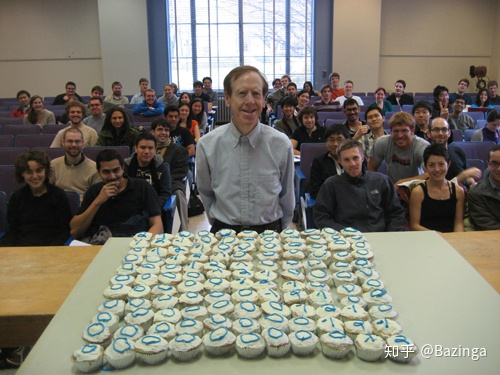
\includegraphics[width=0.6\textwidth]{Gilbert.jpeg}
\end{figure}

\end{frame}

\begin{frame}{Further Study}
\textbf{When finishing this course...}
\vspace{5pt}

Gilbert Strang, MIT, A 2020 Vision of Linear Algebra (Spring 2020)
\url{https://www.bilibili.com/video/BV1GA411t7rL}
\vspace{5pt}

For those who will major in engineering, try these courses:
\begin{itemize}
    \item EE104 Fundamentals of Electric Circuits
    \item MA201b Ordinary Differential Equations B
    \item PHY203-15 Mathematical Methods in Physics
    \item CS405 Machine Learning
\end{itemize}

For those who will major in mathematics, try these courses:
\begin{itemize}
    \item MA109 Advanced Linear Algebra
    \item MA201a Ordinary Differential Equations A
\end{itemize}


\end{frame}

\section{The Geometry of Linear Equations}
\begin{frame}{Linear Equations}


\begin{examples}
Consider this linear equations system with 2 unknowns and 2 equations,
\begin{equation*}
    \begin{cases}
	2x-y=0\\
	-x+2y=3\\
\end{cases}
\end{equation*}
Solve the values of $x$, $y$.
\end{examples}

\textbf{Equivalent Matrix Form:}

\begin{equation*}
    \left[ \begin{matrix}
	2&		-1\\
	-1&		2\\
\end{matrix} \right] \left[ \begin{array}{c}
	x\\
	y\\
\end{array} \right] =\left[ \begin{array}{c}
	0\\
	3\\
\end{array} \right]
\end{equation*}

\begin{equation*}
    A\mathbf{x}=\mathbf{b}
\end{equation*}

Try to understand it in geometric way.
\end{frame}

\begin{frame}{Row Picture}
\vspace{-5pt}
\begin{equation*}
    \begin{cases}
	2x-y=0\\
	-x+2y=3\\
\end{cases}
\end{equation*}

Every row (equation) represents a single straight line.

The problem is to find the intersection of those straight lines.

\begin{figure}
    \centering
    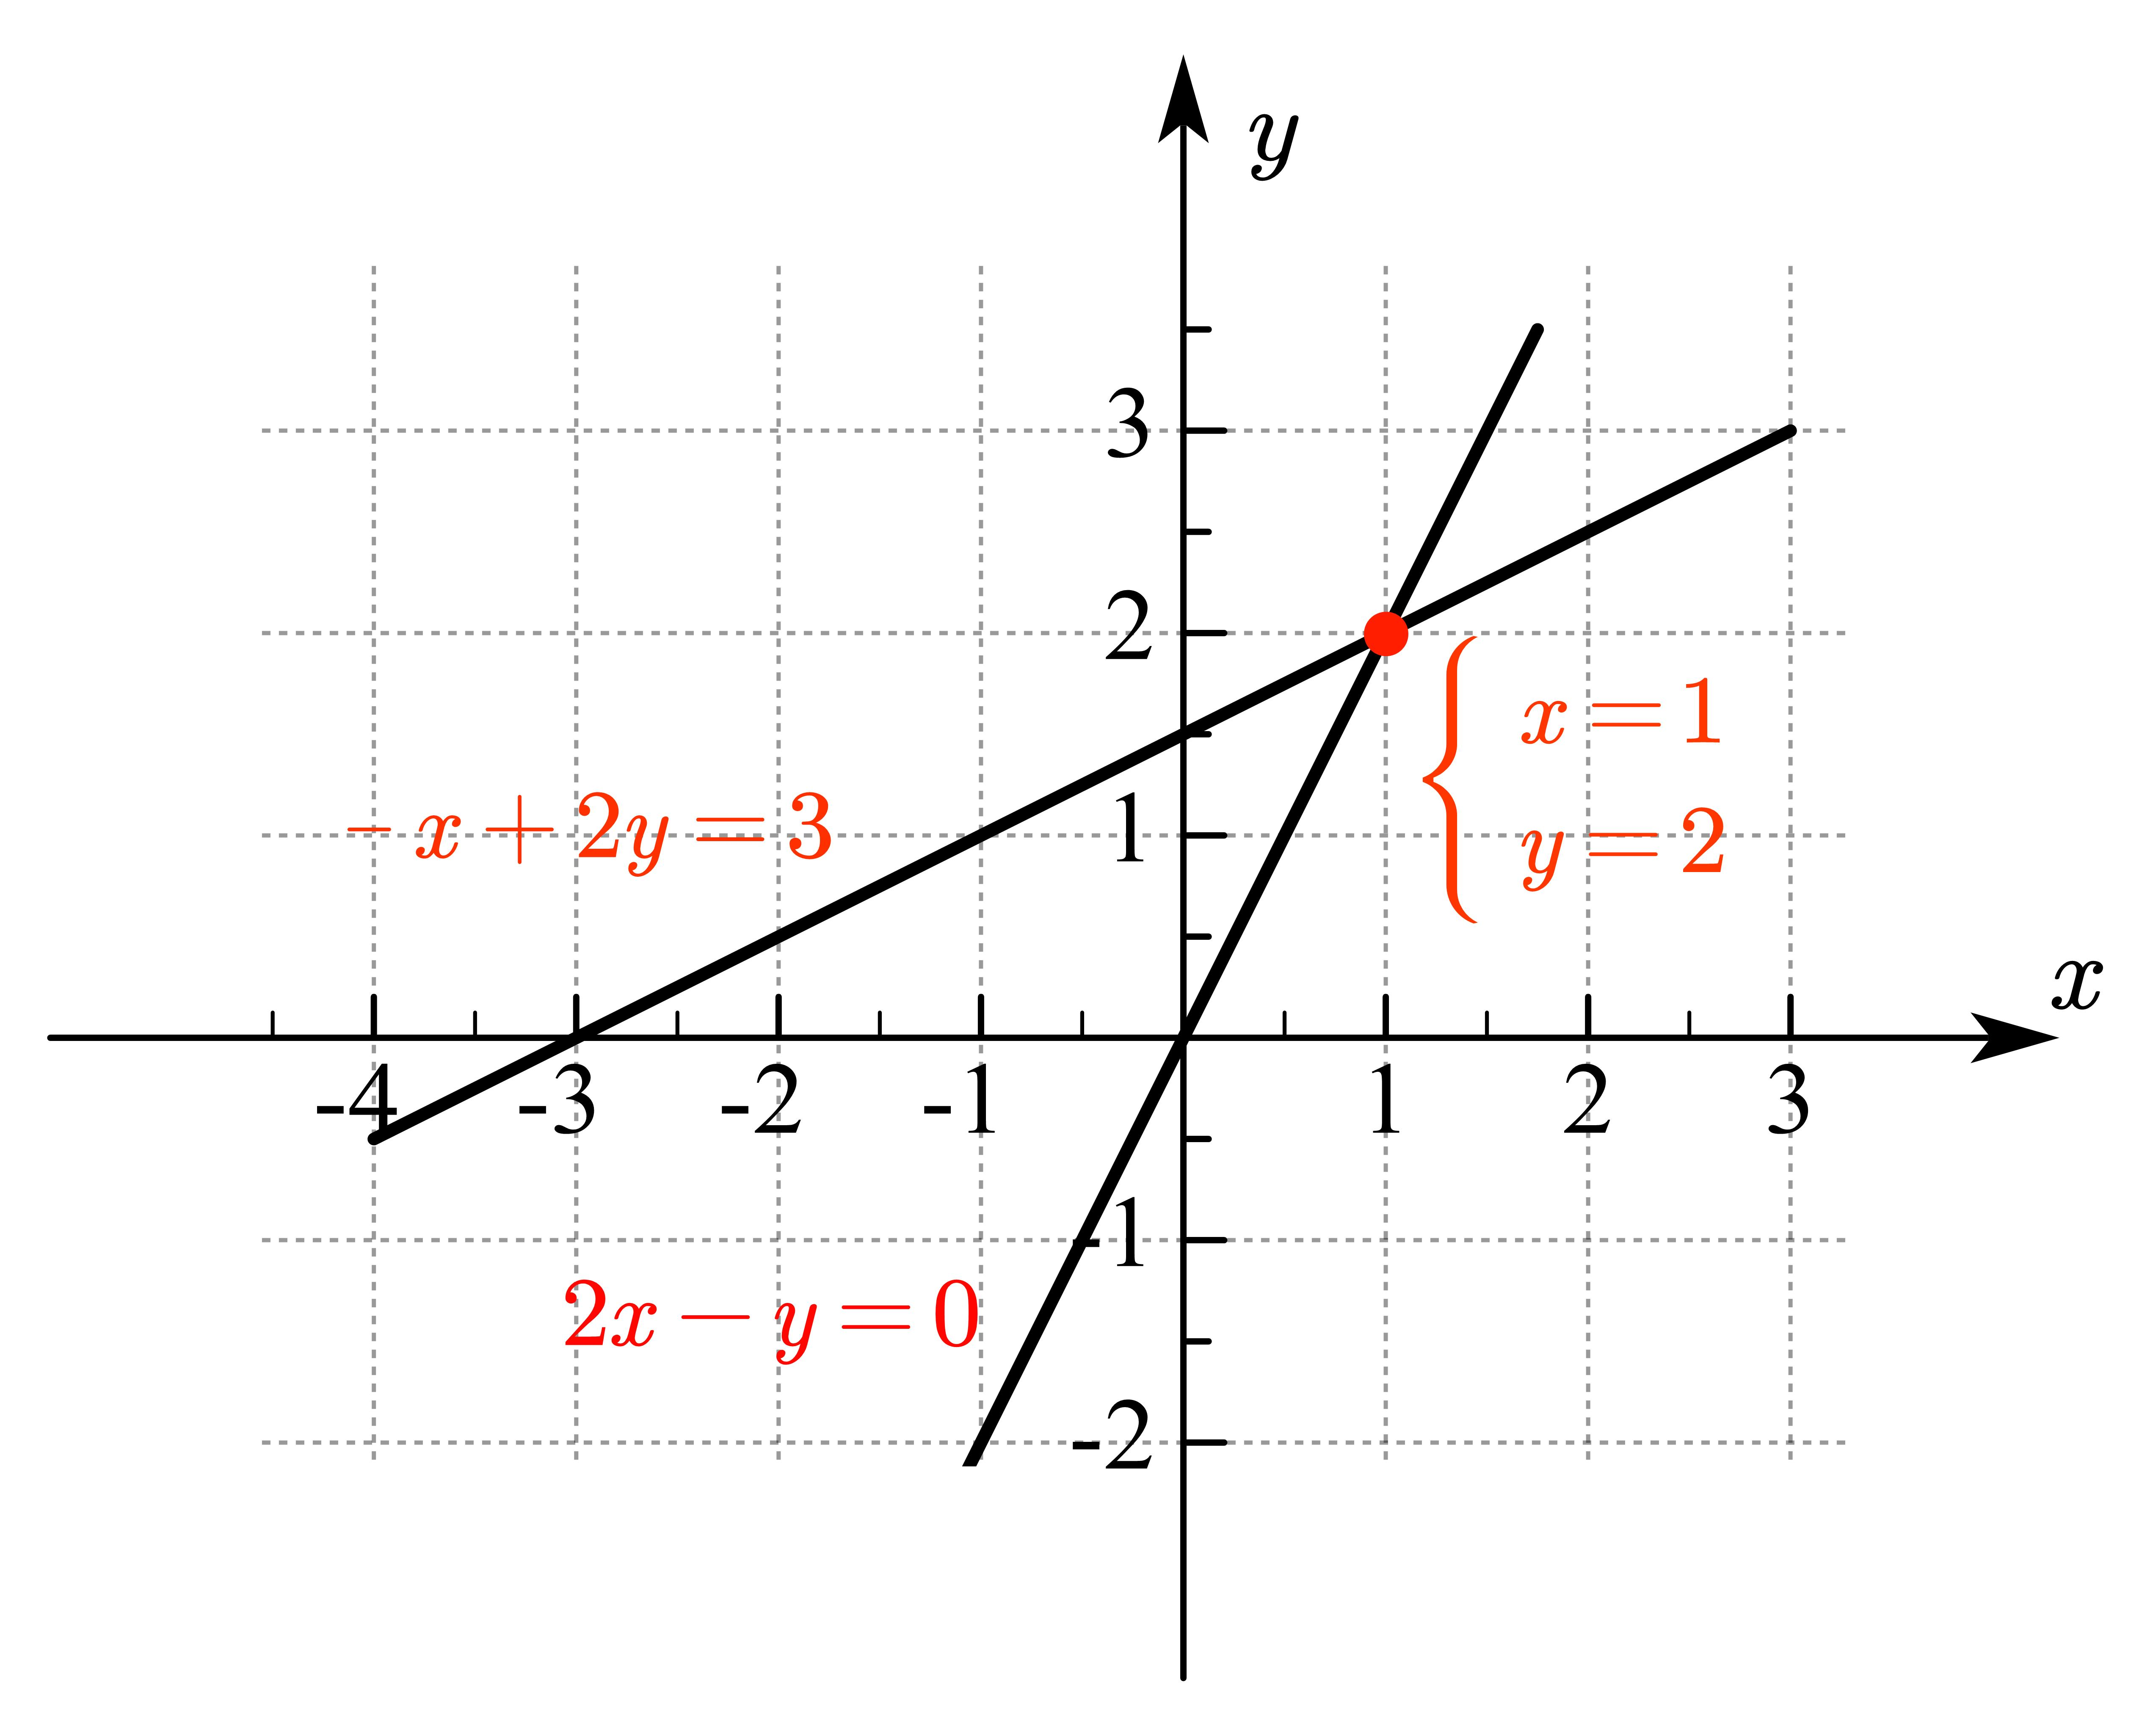
\includegraphics[width=0.55\textwidth]{Row.jpg}
\end{figure}

\end{frame}

\begin{frame}{Column Picture}
\begin{columns}
\column{0.5\textwidth}
\begin{equation*}
    \begin{cases}
	2x-y=0\\
	-x+2y=3\\
\end{cases}
\end{equation*}

\column{0.5\textwidth}
\vspace{-9pt}
\begin{equation*}
    x\left[ \begin{array}{c}
	2\\
	-1\\
\end{array} \right] +y\left[ \begin{array}{c}
	-1\\
	2\\
\end{array} \right] =\left[ \begin{array}{c}
	0\\
	3\\
\end{array} \right]
\end{equation*}
\end{columns}

\vspace{4pt}
Every column (coefficients of a single variable) represents a vector.

The problem is to find the \textbf{Linear Combination} of those vectors.
\vspace{-1.03pt}

\begin{figure}
    \centering
    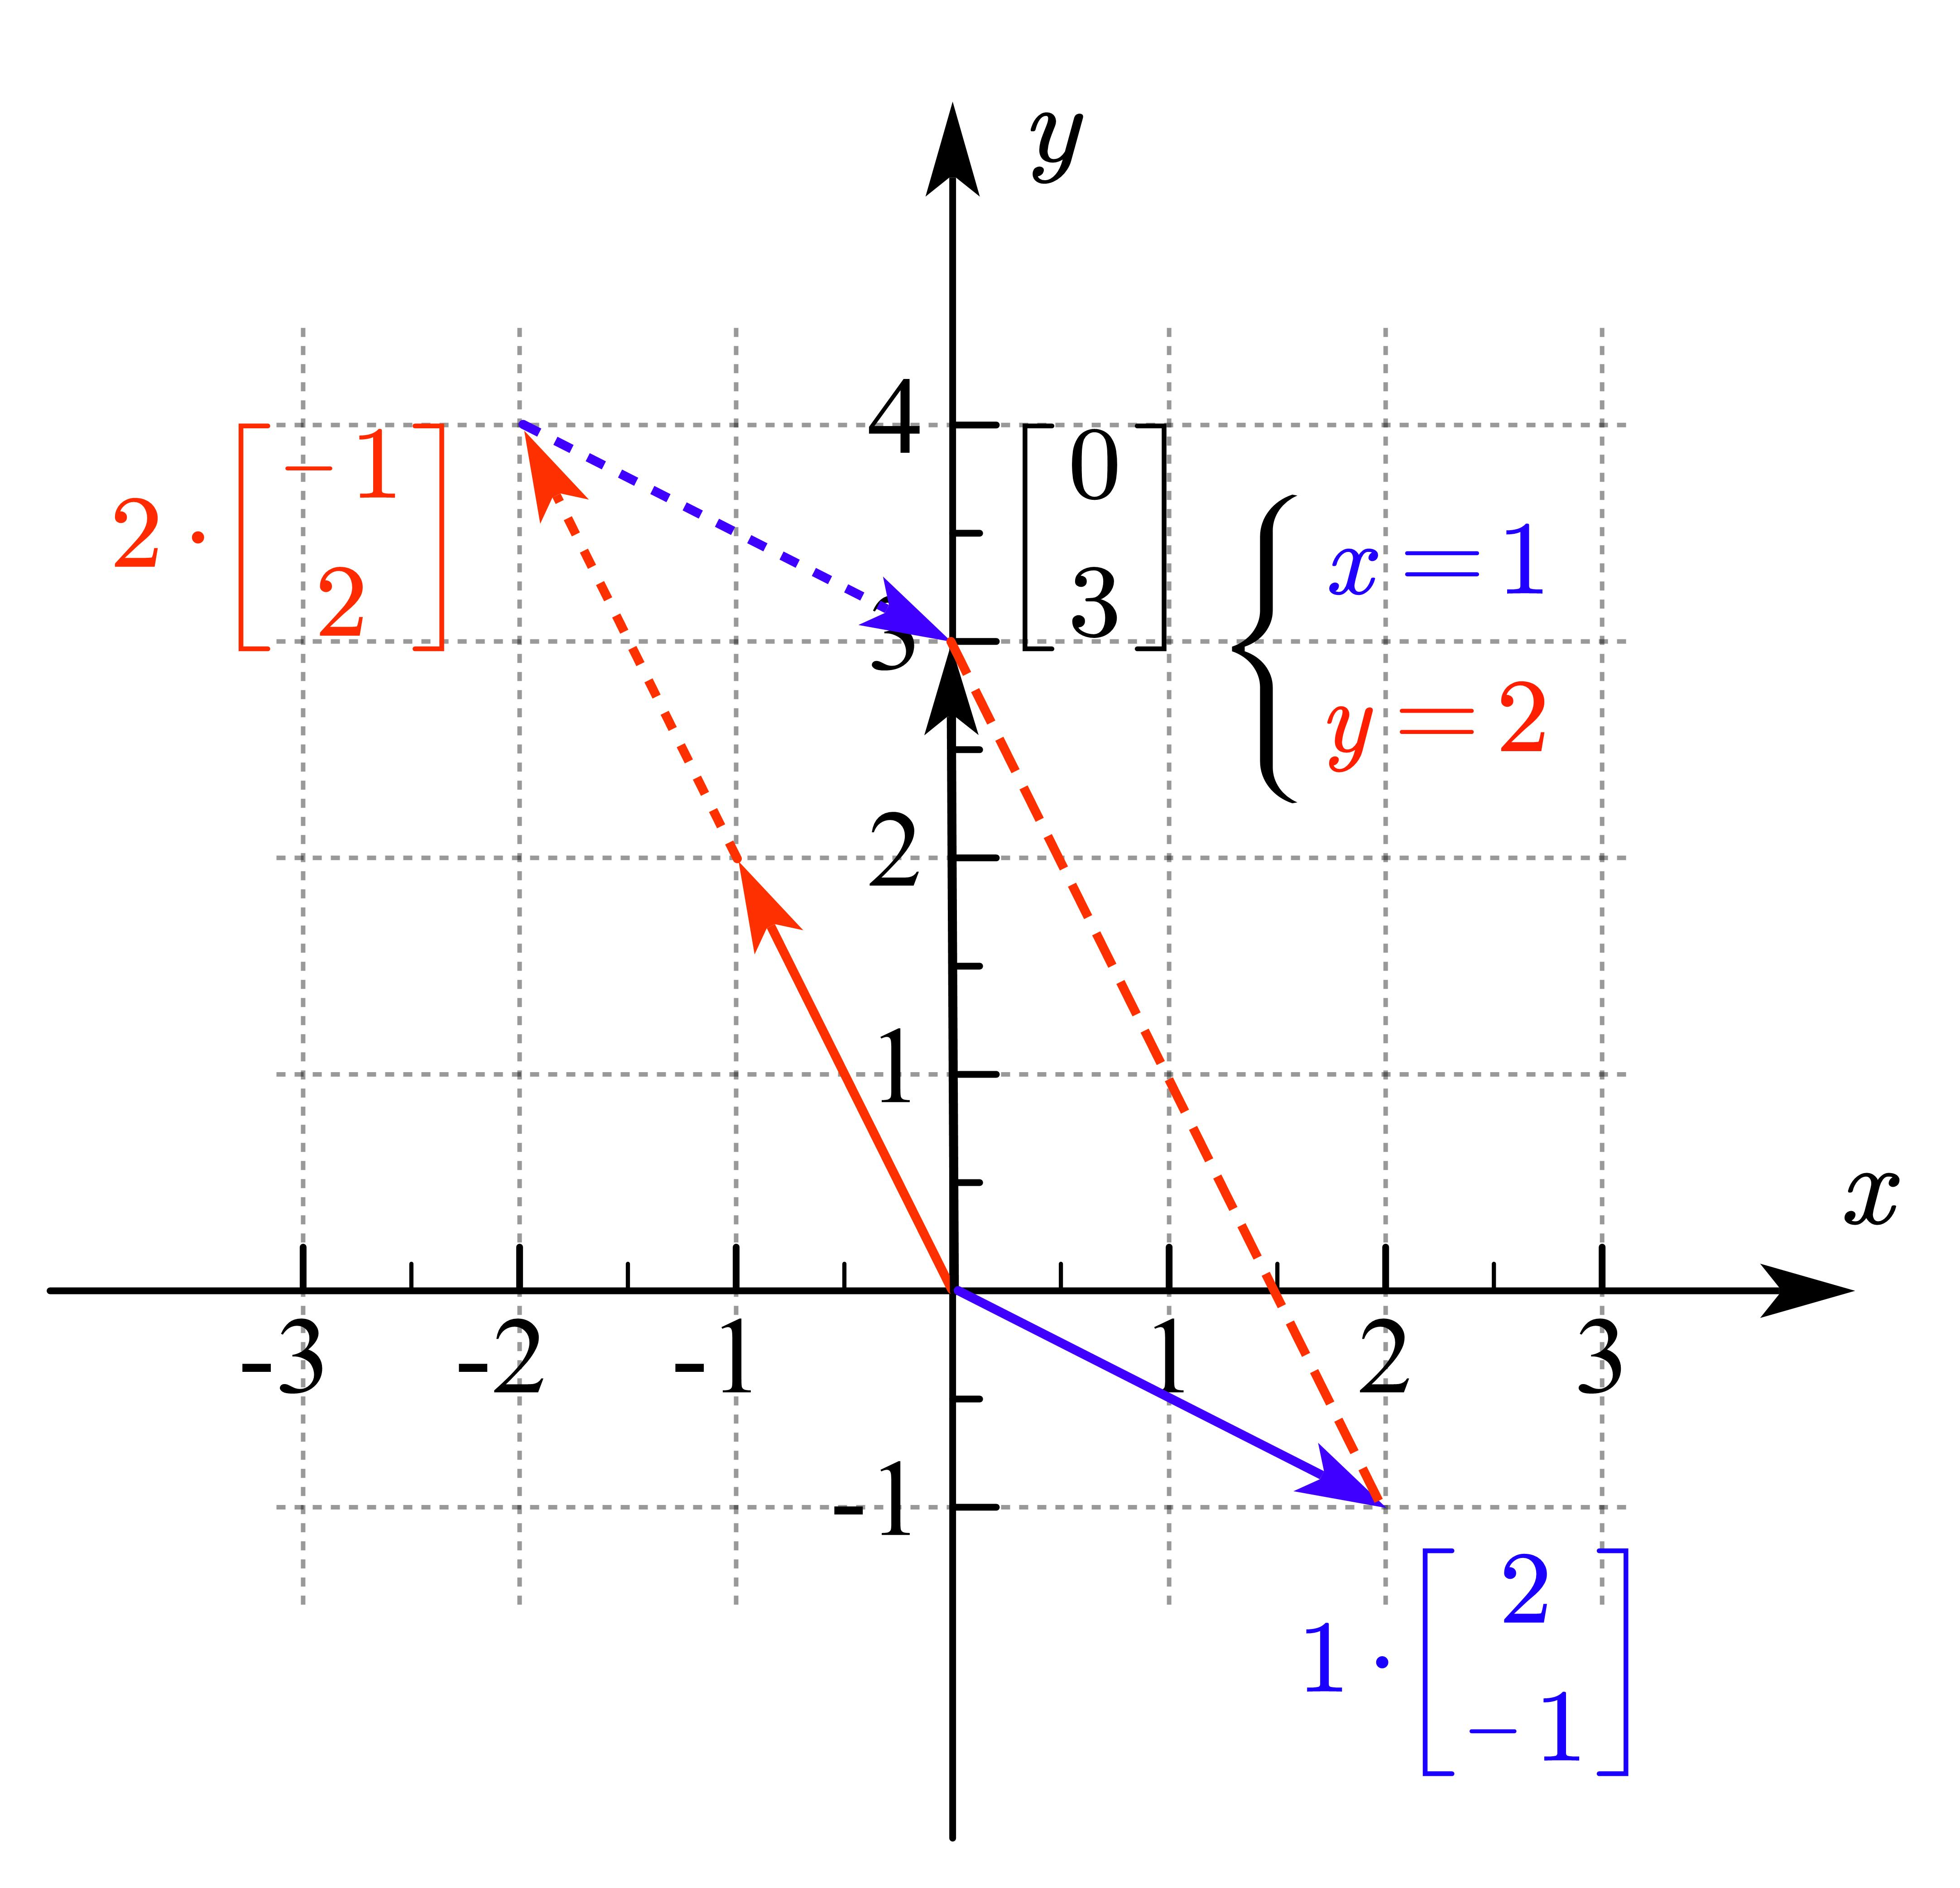
\includegraphics[width=0.48\textwidth]{Column.jpg}
\end{figure}

\end{frame}

\begin{frame}{Gaussian Elimination}
The core problem of linear algebra is to solve linear equations.

Consider the following system of linear equations:

\begin{equation*}
    \begin{cases}
        x+2y+z=2\\
        3x+8y+z=12\\
        4y+z=2\\
    \end{cases}
\end{equation*}

Augmented matrix:
\begin{equation*}
    \left[ \begin{matrix}
        1&		2&		1&		2\\
        3&		8&		1&		12\\
        0&		4&		1&		2\\
    \end{matrix} \right]
\end{equation*}

How can we solve it?
\end{frame}

\begin{frame}{Gaussian Elimination}
Eliminate entry on position $(2,1)$:
\begin{equation*}
    \left[ \begin{matrix}
        1&		2&		1&		2\\
        0&		2&		-2&		6\\
        0&		4&		1&		2\\
    \end{matrix} \right]
\end{equation*}

Eliminate entry on position $(3,1)$:
\begin{equation*}
    (0, skip \: this \: step)
\end{equation*}

Eliminate entry on position $(3,2)$:
\begin{equation*}
    \left[ \begin{matrix}
        1&		2&		1&		2\\
        0&		2&		-2&		6\\
        0&		0&		5&		-10\\
    \end{matrix} \right]
\end{equation*}

Elimination process done! Find the pivots above.
\end{frame}


\begin{frame}{Back-Substitution}
After elimination, we get
\begin{columns}
    \column{0.5\textwidth}
    \begin{equation*}
        \left[ \begin{matrix}
            1&		2&		1&		2\\
            0&		2&		-2&		6\\
            0&		0&		5&		-10\\
        \end{matrix} \right]
    \end{equation*}

    \column{0.5\textwidth}
    \begin{equation*}
        \begin{cases}
            x+2y+z=2\\
            2y-2z=6\\
            5z=-10\\
        \end{cases}
    \end{equation*}
\end{columns}
Do back-substitution, we can get the solution:
\begin{equation*}
    \begin{cases}
        x=2\\
        y=1\\
        z=-2\\
    \end{cases}
\end{equation*}

Rethink the whole elimination process, are there exist some cases to let the elimination process break down?
\end{frame}

\begin{frame}{Singular Cases for Gauss Elimination}
The matrix we used above is a "good" matrix.
\begin{equation*}
    \left[ \begin{matrix}
        1&		2&		1&		2\\
        3&		8&		1&		12\\
        0&		4&		1&		2\\
    \end{matrix} \right]
\end{equation*}

If we slightly change one of the element\dots
\begin{equation*}
    \left[ \begin{matrix}
        1&		2&		1&		2\\
        3&		6&		1&		12\\
        0&		4&		1&		2\\
    \end{matrix} \right]
\end{equation*}

What will happen now?
\end{frame}

\begin{frame}{Singular Cases for Gauss Elimination}
Eliminate entry on position $(2,1)$:
\begin{equation*}
    \left[ \begin{matrix}
        1&		2&		1&		2\\
        0&		0&		-2&		6\\
        0&		4&		1&		2\\
    \end{matrix} \right]
\end{equation*}

Eliminate entry on position $(3,1)$:
\begin{equation*}
    (0, skip \: this \: step)
\end{equation*}

Eliminate entry on position $(3,2)$:
\begin{equation*}
    Something \: strange \: happens.
\end{equation*}

Elimination process fails! Missing pivots.

Method to solve: Row exchange.
\end{frame}

\begin{frame}{Singular Cases for Gauss Elimination}
Another change to make the "good" matrix singular:
\begin{equation*}
    \left[ \begin{matrix}
        1&		2&		1&		2\\
        3&		8&		1&		12\\
        0&		4&		-4&		2\\
    \end{matrix} \right]
\end{equation*}

Eliminate entry on position $(2,1)$:
\begin{equation*}
    \left[ \begin{matrix}
        1&		2&		1&		2\\
        0&		2&		-2&		6\\
        0&		4&		-4&		2\\
    \end{matrix} \right]
\end{equation*}

Eliminate entry on position $(3,2)$:
\begin{equation*}
    \left[ \begin{matrix}
        1&		2&		1&		2\\
        0&		2&		-2&		6\\
        0&		0&		0&		-10\\
    \end{matrix} \right]
\end{equation*}

Elimination fails. Missing pivots. No method to fix.

\end{frame}






\begin{frame}{Linear Transfomations}
How to determine whether a transformation is linear?

\vspace{5pt}
Two rules:
\begin{itemize}
    \item Origin remains unchanged.
    \item Straight lines are still straight lines.
\end{itemize}

Generalize it and express in mathematical languages, a mapping $T$ is a linear transformation if
\begin{enumerate}
    \item $T\left( \mathbf{u}+\mathbf{v} \right) =T\left( \mathbf{u} \right) +T\left( \mathbf{v} \right)$
    \item $T\left( \alpha \mathbf{v} \right) =\alpha T\left( \mathbf{v} \right) $
\end{enumerate}
\end{frame}

\begin{frame}{Matrix as Linear Transformation}
See this example of Linear Transformation:


To fully express a Linear Transformation, we can track the movement of two random vectors. Since we know that every vector in $\mathbb{R}^2$ space can be expressed by these 2 vectors!
\end{frame}

\begin{frame}{Matrix as Linear Transformation}
\vspace{-3pt}
Track the two unit vectors (the red one and the green one).
\vspace{3pt}
\begin{columns}
\column{0.5\textwidth}
\hspace{5pt}Before transformation:
\vspace{-3pt}
\begin{equation*}
    \boldsymbol{\hat{i}}=\left[ \begin{array}{c}
	1\\
	0\\
\end{array} \right] ,  \boldsymbol{\hat{j}}=\left[ \begin{array}{c}
	0\\
	1\\
\end{array} \right]
\end{equation*}

\column{0.5\textwidth}
\hspace{5pt}After transformation:\
\vspace{-3pt}
\begin{equation*}
    T(\boldsymbol{\hat{i}})=\left[ \begin{array}{c}
	2\\
	1\\
\end{array} \right] ,  T(\boldsymbol{\hat{j}})=\left[ \begin{array}{c}
	0\\
	1\\
\end{array} \right]
\end{equation*}
\end{columns}
\vspace{3pt}
Then the linear transformation can be expressed by a matrix:
    \begin{equation*}
        A= \left[ \begin{matrix}
    	2&		0\\
    	1&		1\\
    \end{matrix} \right] ,
    \end{equation*}

where the first column is the vector $\boldsymbol{\hat{i}}$ after transformation, the second column is the vector $\boldsymbol{\hat{j}}$ after transformation.
\end{frame}

\begin{frame}{Matrix as Linear Transformation}


\begin{columns}
\column{0.5\textwidth}
\vspace{-3pt}

\column{0.5\textwidth}
\vspace{-3pt}
\end{columns}



Now we focus on another vector, the yellow one for instance.

\begin{itemize}
    \item Before Linear Transformation, the vector can be expressed as the linear combinations of $\boldsymbol{\hat{i}} , \boldsymbol{\hat{j}}$.

\vspace{-10pt}
\begin{equation*}
\mathbf{x}=\boldsymbol{\hat{i}}+2\boldsymbol{\hat{j}}
=\left[ \begin{array}{c}
	1\\
	0\\
\end{array} \right] +2\left[ \begin{array}{c}
	0\\
	1\\
\end{array} \right] =\left[ \begin{array}{c}
	1\\
	2\\
\end{array} \right] =\left[ \begin{matrix}
	1&		0\\
	0&		1\\
\end{matrix} \right] \left[ \begin{array}{c}
	1\\
	2\\
\end{array} \right]
\end{equation*}

    \item After Linear Transformation, the relation of $\mathbf{x}=\boldsymbol{\hat{i}}+2\boldsymbol{\hat{j}}$ still exists, which can be proved by the definition of Linear Transformation.

\vspace{-12.1pt}
\begin{equation*}
T(\mathbf{x})=T(\boldsymbol{\hat{i}})+2T(\boldsymbol{\hat{j}})=
\left[ \begin{array}{c}
	2\\
	1\\
\end{array} \right] +2\left[ \begin{array}{c}
	0\\
	1\\
\end{array} \right] =\left[ \begin{array}{c}
	2\\
	3\\
\end{array} \right] =\left[ \begin{matrix}
	2&		0\\
	1&		1\\
\end{matrix} \right] \left[ \begin{array}{c}
	1\\
	2\\
\end{array} \right]
\end{equation*}

\end{itemize}
\end{frame}

\begin{frame}{See Linear Transformation in Two Perspectives}
\begin{itemize}
    \item In geometrical perspective of view, linear transformation is a mapping rule $T$, i.e. a function of vectors.
    \begin{equation*}
    \mathbf{v}\in V\xrightarrow{\mathrm{Transformation \,T}}\mathbf{w}=T\left( \mathbf{v} \right) \in W      
    \end{equation*}
    \item In algebraic perspective of view, linear transformation is to left multiply a transformation matrix $A$.
    \begin{equation*}
    \mathbf{v}\in V\xrightarrow{\mathrm{Transformation \,Matrix \,A}}T\left( \mathbf{v} \right)=A\mathbf{v} \in W      
    \end{equation*}
\end{itemize}

Now, you may easily verify the following expression using geometrical perspective of view.
\begin{equation*}
    A^{12}=\left[ \begin{matrix}
	\frac{\sqrt{3}}{2}&		-\frac{1}{2}\\
	\frac{1}{2}&		\frac{\sqrt{3}}{2}\\
\end{matrix} \right] ^{12}=\left( \begin{matrix}
	1&		0\\
	0&		1\\
\end{matrix} \right) =I
\end{equation*}
Rotate 30 degrees by 12 times, the plane remains unchanged.
\end{frame}



\section{Chapter 5.1: Eigenvalues and Eigenvectors}

\begin{frame}{Eigenvalues and Eigenvectors}
After Linear Transformation, almost all the vectors will have changes in both direction and magnitude as following.


However, there exist some special cases a vector's direction will not change after the linear transformation.

\end{frame}

\begin{frame}{Eigenvalues and Eigenvectors}
Use algebraic perspective of view to describe the linear transformation above:
\begin{equation*}
    \left[ \begin{matrix}
	3&		1\\
	0&		2\\
\end{matrix} \right] \left[ \begin{array}{c}
	1\\
	-1\\
\end{array} \right] =\left[ \begin{array}{c}
	3\\
	0\\
\end{array} \right] -\left[ \begin{array}{c}
	1\\
	2\\
\end{array} \right] =\left[ \begin{array}{c}
	2\\
	-2\\
\end{array} \right] =2\left[ \begin{array}{c}
	1\\
	-1\\
\end{array} \right]
\end{equation*}

Then we can define $\lambda =2$ as the eigenvalue, $\left[ \begin{array}{c}
	1\\
	-1\\
\end{array}\right]$ as the eigenvector corresponding to this eigenvalue.
\end{frame}

\begin{frame}{Eigenvalues and Eigenvectors}
\begin{block}{Definition}
    Let $A$ be a square matrix of degree $n$. If there exist a non-zero vector $\mathbf{x}$ and a scalar $\lambda$ such that
    \begin{equation*}
        A \mathbf{x}=\lambda \mathbf{x},
    \end{equation*}
    then $\lambda$ is called an \alert{eigenvalue} of $A$, and $\mathbf{x}$ is called an \alert{eigenvector} corresponding to the eigenvalue $\lambda$ .
\end{block}
\begin{block}{Remark}
    The zero vector can not be an eigenvector even though $A0=\lambda 0$, but $\lambda=0$ can be an eigenvalue.
\end{block}

\end{frame}

\begin{frame}{Understanding Eigenvalues in Geometry}
\begin{equation*}
    A \mathbf{x}=\lambda \mathbf{x}
\end{equation*}
$A \mathbf{x}$: the vector $\mathbf{x}$ after linear transformation.

$\lambda \mathbf{x}$: real multiples of $\mathbf{x}$, i.e. stretching of vector $\mathbf{x}$.

The linear transformation for \textit{eigenvector} result in stretching the vector by \textit{eigenvalue} times.
\end{frame}

\begin{frame}{Calculating Eigenvalues and Eigenvectors}
How about understanding stretching another linear transformation?
\begin{equation*}
    A \mathbf{x}=\lambda I \,\mathbf{x}
\end{equation*}

The two linear transformations for vector $\mathbf{x}$ are equivalent, leading
\begin{equation*}
    \left(A-\lambda I \right) \mathbf{x}=0.
\end{equation*}

Therefore, vector $\mathbf{x}$ is in the nullspace of matrix $\left(A-\lambda I \right)$. To make this linear equation have nonzero solutions (i.e. to make the dimension of nullspace not zero), matrix $\left(A-\lambda I \right)$ should not be a full rank matrix. Expressed in determinant form:

\begin{equation*}
    \det \left( A-\lambda I \right) =0
\end{equation*}
\end{frame}


\begin{frame}{Calculating Eigenvalues and Eigenvectors}
\begin{examples}
Calculate the eigenvalues and eigenvectors of matrix A.
\begin{equation*}
    A=\left[ \begin{matrix}
	4&		-5\\
	2&		3\\
\end{matrix} \right]
\end{equation*}
\end{examples}
\textbf{Solution:}
\begin{equation*}
    \det \left( A-\lambda I \right) =\left| \begin{matrix}
	4-\lambda&		-5\\
	2&		-3-\lambda\\
\end{matrix} \right|=\left( \lambda -2 \right) \left( \lambda +1 \right) =0
\end{equation*}

For eigenvalue $\lambda_1=2$,
\begin{equation*}
    \left( A-\lambda I \right) \mathbf{x}=\left[ \begin{matrix}
	2&		-5\\
	2&		-5\\
\end{matrix} \right] \left[ \begin{array}{c}
	x_1\\
	x_2\\
\end{array} \right] =\left[ \begin{array}{c}
	0\\
	0\\
\end{array} \right] , \, \mathbf{x}=k\left[ \begin{array}{c}
	5\\
	2\\
\end{array} \right]
\end{equation*}

Eigenvectors corresponding to $\lambda_1=2$ are of the form $\mathbf{x}=k\left[ \begin{array}{c}
	5\\
	2\\
\end{array} \right],\,k\ne 0$

The same process for another eigenvalue $\lambda_2=-1$
\end{frame}
\end{document}